\documentclass[12pt]{article}


\usepackage{sbc-template}

\usepackage[utf8]{inputenc}
\usepackage{textcomp}
\usepackage{graphicx,url}

%\usepackage[brazil]{babel}   
%\usepackage[latin1]{inputenc}  

     
\sloppy

\title{Módulos generativos em SInCoPA - Técnicas e idéias musicais em um sistema de música interativa}

\author{autor}


\address{Universidade
  (UF)\\
    Brazil
  \email{e-mail@autor}
}

\begin{document} 

\maketitle

\begin{abstract}
  In this article I will address one part of the development
my personal system of composition, performance and
analysis (SInCoPA). The system goal is to help
the creation of interactive music where one seeks
polyphony with a dense texture variations
in dialogues with the computer player.
Throughout the text I will present the modules of algorithms
generative designed to work in sync
with the analysis of real-time audio.
SInCoPA is built with the language Pure Data (Pd).
An important aspect is the visualization of images
of patches that have all the details of implementation
code.
Some ideas and implementations are explained
detail so that it can rebuild
the system through the documentation.

\end{abstract}
     
\begin{resumo} 
  Nesse artigo irei abordar uma parte do desenvolvimento
de meu sistema pessoal de composição, performance e
análise (SInCoPA). O objetivo do sistema é auxiliar
na criação de música interativa onde se busca
uma polifonia densa com variações de textura
nos diálogos do instrumentista com o computador.
Ao longo do texto vou apresentar os módulos de algoritmos
generativos criados para trabalhar em sincronia
com a análise de áudio em tempo-real.
SInCoPA é construído com a linguagem Pure data (Pd).
Um importante aspecto é a vizualização das imagens
dos patchs que apresentam todos os detalhes de implementação
do código.
Algumas idéias e implementações são explicadas
detalhadamente de maneira que se possa reconstruir
o sistema através da documentação.


\end{resumo}


\section{Geradores algorítmicos}

Durante a implementação dos geradores de material musical,
procurou-se aliar técnicas de composição algorítmica com
o resultado das análises do áudio de entrada.

A idéia é de ter uma coleção de geradores, capazes
de imitar, simular, seguir ou serem alterados por elementos da performance humana. A análise do áudio
tenta fazer uma descrição da performance e essa descrição
é enviada aos geradores, mediados pelo cenário de interação.
Nesse sentido as análises alimentam os parâmetros dos
geradores, conduzindo o comportamento dos mesmos.

Notadamente alguns trabalhos tem influenciado bastante o desenvolvimento
dos geradores, servindo de ponto de partida para a implementação. Como
por exemplo a biblioteca RTC\footnote{A biblioteca RTC (\textit{Real-Time Composition} 
foi desenvolvida pelo compositor Karlheinz Essl em MAX, a re-implementação
em Pd foi feita por Frank Barchnet, poderemos ver uma visão mais geral
das funcionalidades dessa biblioteca no apêndice} e o método MEPSOM\footnote{
MEPSOM (Método de Ensino de Programação Sônica para Músicos) desenvolvido por
Elói Fritsch é um método que ensina composição algorítmica no ambiente MAX. Alguns
exemplos de MEPSOM foram portados para Pd e podem ser vistos no apêndice}, além
de alguns objetos das bibliotecas PDMTL e Rj.  

Músicos frequentemente separam os aspectos rítmicos, melódicos e de dinâmica
quando estudam performance ou compõe. É comum um instrumentista executar um 
mesmo perfil melódico em diferentes combinações rítmicas e com articulações
diferentes. Muitos métodos de educação musical começam com exercícios rítmicos
para depois incluir exercícios melódicos. Ao implementar os geradores midi
nessa pesquisa, levou-se em conta esses aspectos e decidiu-se manter a separação
entre os domínios do ritmo, melodia e dinâmica. Criando uma relação de funcionamento
desses geradores, possibilitando uma expansão organizada de técnicas de geração.
Na implementação de Sincopa, projetamos 3 objetos que trabalham sincronizados para
gerar alturas, amplitudes e durações respectivamente.

Cada um desses objetos gerencia algumas técnicas de geração
algorítmica. É possível qualquer combinação entre esses três objetos.
A combinação entre os diversos geradores se dá na relação entre a 
análise do áudio de entrada e a escolha de um cenário de interação. 
Cada uma dessas dimensões administra geradores que se enquadram nas seguintes
categorias:

\begin{itemize}
 \item   Imitação
 \item   Variação
 \item   Movimento browniano
 \item   Probabilidade
 \item   Randômico
 \item   Boids
\end{itemize}

Qualquer combinação dessas categorias com a performance do músico guarda, a priori,  
uma relação de unidade composicional por se basear no material fornecido pelo músico.
Mas claramente, após a análise de cada algoritmo, iremos notar que algumas combinações 
geram uma ``sensação'' de unidade mais forte que outras. Apesar dessa pesquisa
não se ocupar com problemas de pesquisa em cognição, algumas conclusões advindas
do manuseio e experimentação das ferramentas apresentadas podem ser apontadas.

Por exemplo, se o gerador rítmico for imitativo, o melódico baseado em
variação e o gerador de amplitude for randômico, vamos obter um resultado
com forte unidade composicional pois a dimensão rítmica contribui intensamente
para essa sensação de unidade. Numa performance de música interativa essa sensação
de unidade é importante para o músico que está interagindo com a máquina. Criando
pontos de apoio na narrativa global, onde o músico consegue controlar musicalmente 
aspectos do diálogo. Podemos inferir que essa sensação de unidade está relacionada
a sensação de controle do discurso, no caso do músico atuando em uma sessão de música
interativa.


\subsection{Variação}
\label{varia-contorno}

%% aqui incluir operações de contorno
%% operações em arrays (transposição, inversão, retrógrado , rotação, normalização) - gerando midi

Denominamos variação um procedimento que toma como base um
material dado e aplica uma operação de transformação nesse material.
Nessa pesquisa, o material de base são os próprios dados da 
análise da performance musical.
Aqui serão descritos algumas técnicas de variação melódica como
transposição, inversão, retrogradação e também de variação rítmica
como expansão e contração de durações. Além de outras possibilidades
de leitura de arrays e transformações.

\begin{figure}
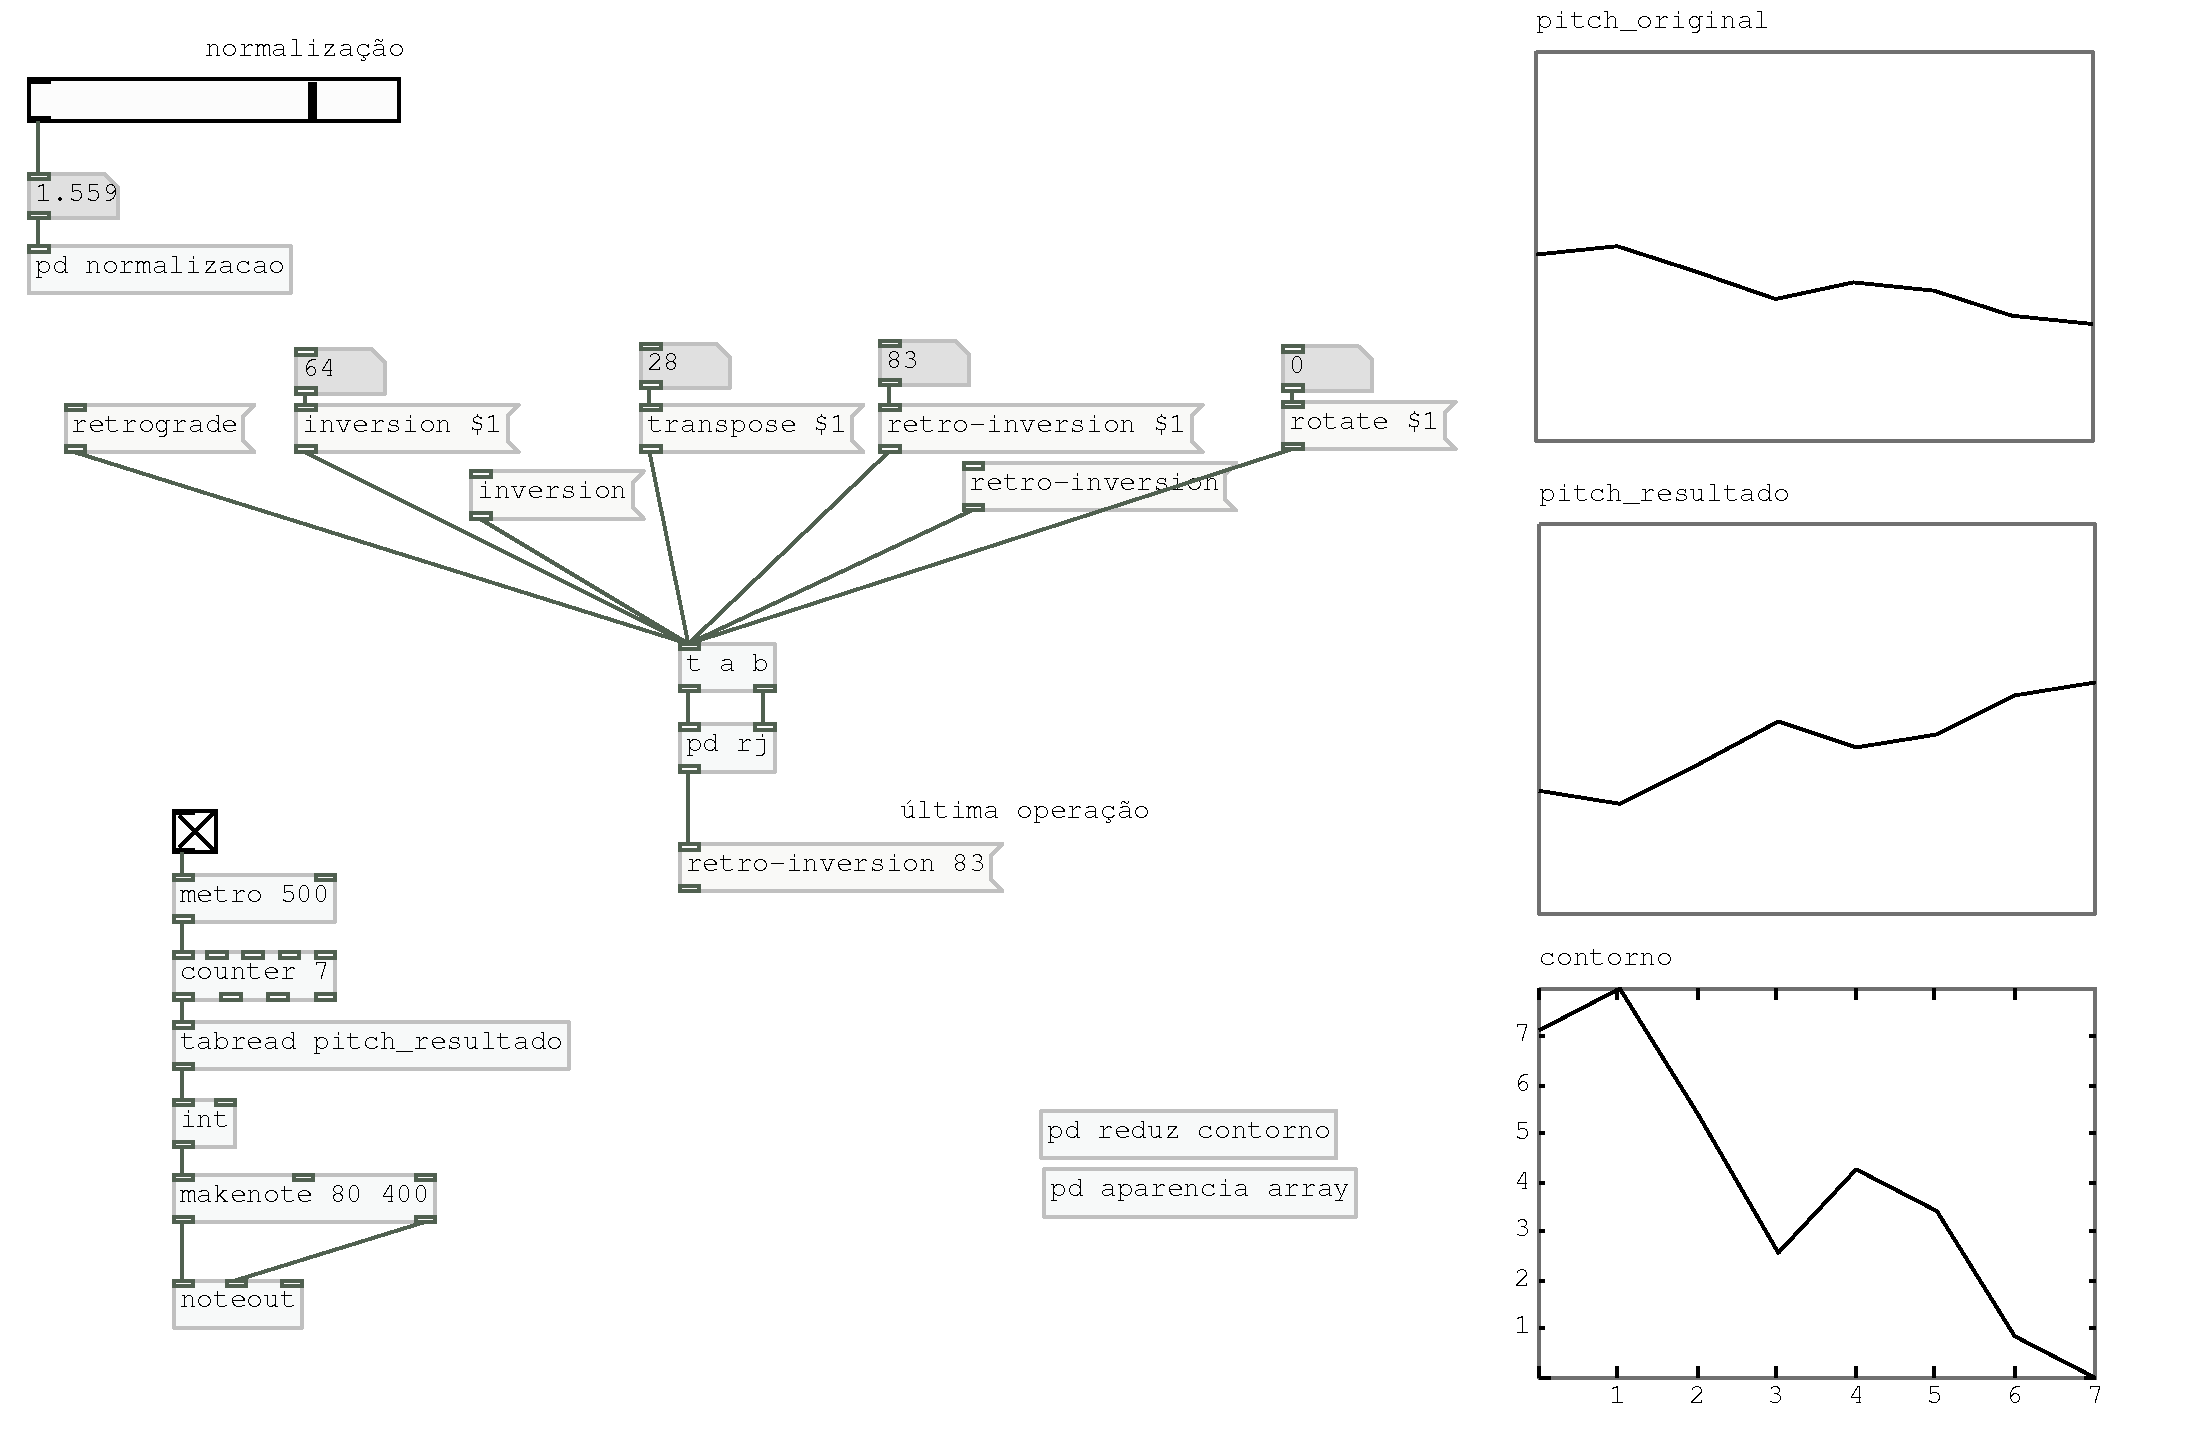
\includegraphics[scale=.6]{variacoes-contorno}
\caption{Patch mostrando operações de variação sobre array}
\label{variacoes-contorno}
\end{figure}  

Na figura \ref{variacoes-contorno} vemos acima um array ``pitch\_original'' que representa
o conjunto de pitches executados pelo músico (poderia ser durações ou qualquer
outro parâmetro). Abaixo, no centro, o array ``pitch\_resultado'' mostrando o resultado das  
operações de variação. E abaixo, um array ``contorno'' mostrando a redução do contorno em
``pitch\_original'' para a forma normal, como visto em \cite{sampaio08:torno}.


Podemos aplicar a operação de transposição ao parâmetro
de durações das notas, obtendo o efeito de expansão e contração
rítmica, bastante utilizados em técnicas de contraponto tonal.



\subsection{Movimento browniano}

%% ver rowe pg 306

O objeto [brown-rhythm] está presente na biblioteca RTC e se trata de
um gerador de durações baseado em movimento browniano("Brown motion"
\footnote{movimento browniano é um modelo que descreve o movimento aleatório 
de partículas macroscópicas num fluido como consequência dos choques das 
moléculas das partículas. Esse nome é devido ao botânico Robert
Brown, que observou minúsculas partículas dentro dos vacúolos dos grãos de 
pólen executando um movimento agitado. Repetindo o experimento com partículas de poeira, 
ele foi capaz de definir que o movimento se deu devido às partículas estarem "vivas", 
embora a origem do movimento ainda estivesse para ser explicada.
O cientista que explicou corretamente esse movimento, propondo que a energia fosse 
constituída de partículas, foi Albert Einstein, em 1905.
Movimento browniano é um dos modelos mais usados de processos estocásticos
(ou probabilísticos) sobre tempo contínuo.} )

 \begin{figure}
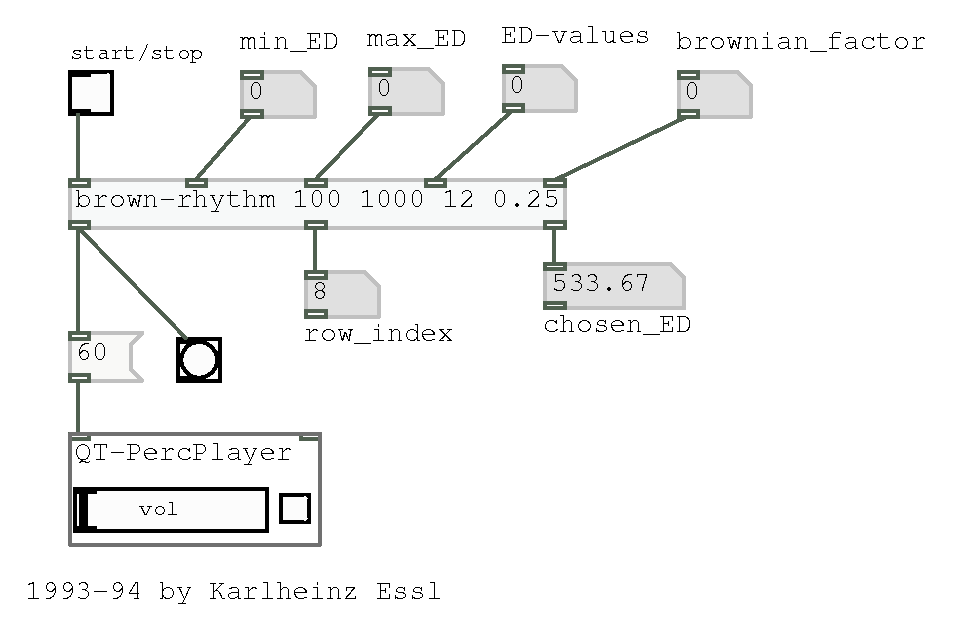
\includegraphics[scale=.6]{brown-rhythm-func}
\caption{Funcionamento básico de [brow-rhythm]}
\label{brown-rythm-func}
\end{figure} 

No manual de [brown-rhythm] aparece uma explicação mais detalhada.


\begin{quote}
Generates a brownian-movement-like rhythm of a geometrical row of
entry delays (ED) and a certain number of ED-values. The brownian factor
determines the distance between two succeding rhythmical values. A factor
of 0 produces a periodic rhythm, where a factor of 1 output random values 
of the given range.
\end{quote}  


Podemos ver o funcionamento básico do objeto [brownian] acessando seu
manual (figura \ref{brownian-func}.  A saída desse objeto retorna números randômicos entre o mínimo
(''min'' (int, float)) e o máximo (''max" (int, float)). A distância entre
dois números randômicos é determinada pelo fator de brown (float
entre 0 e 1). Quando esse fator é 1, [brownian] se comporta como um
gerador randômico ordinário (objeto [random] por exemplo). Quando
o fator é 0, o mesmo número sempre é repetido.


\begin{figure}
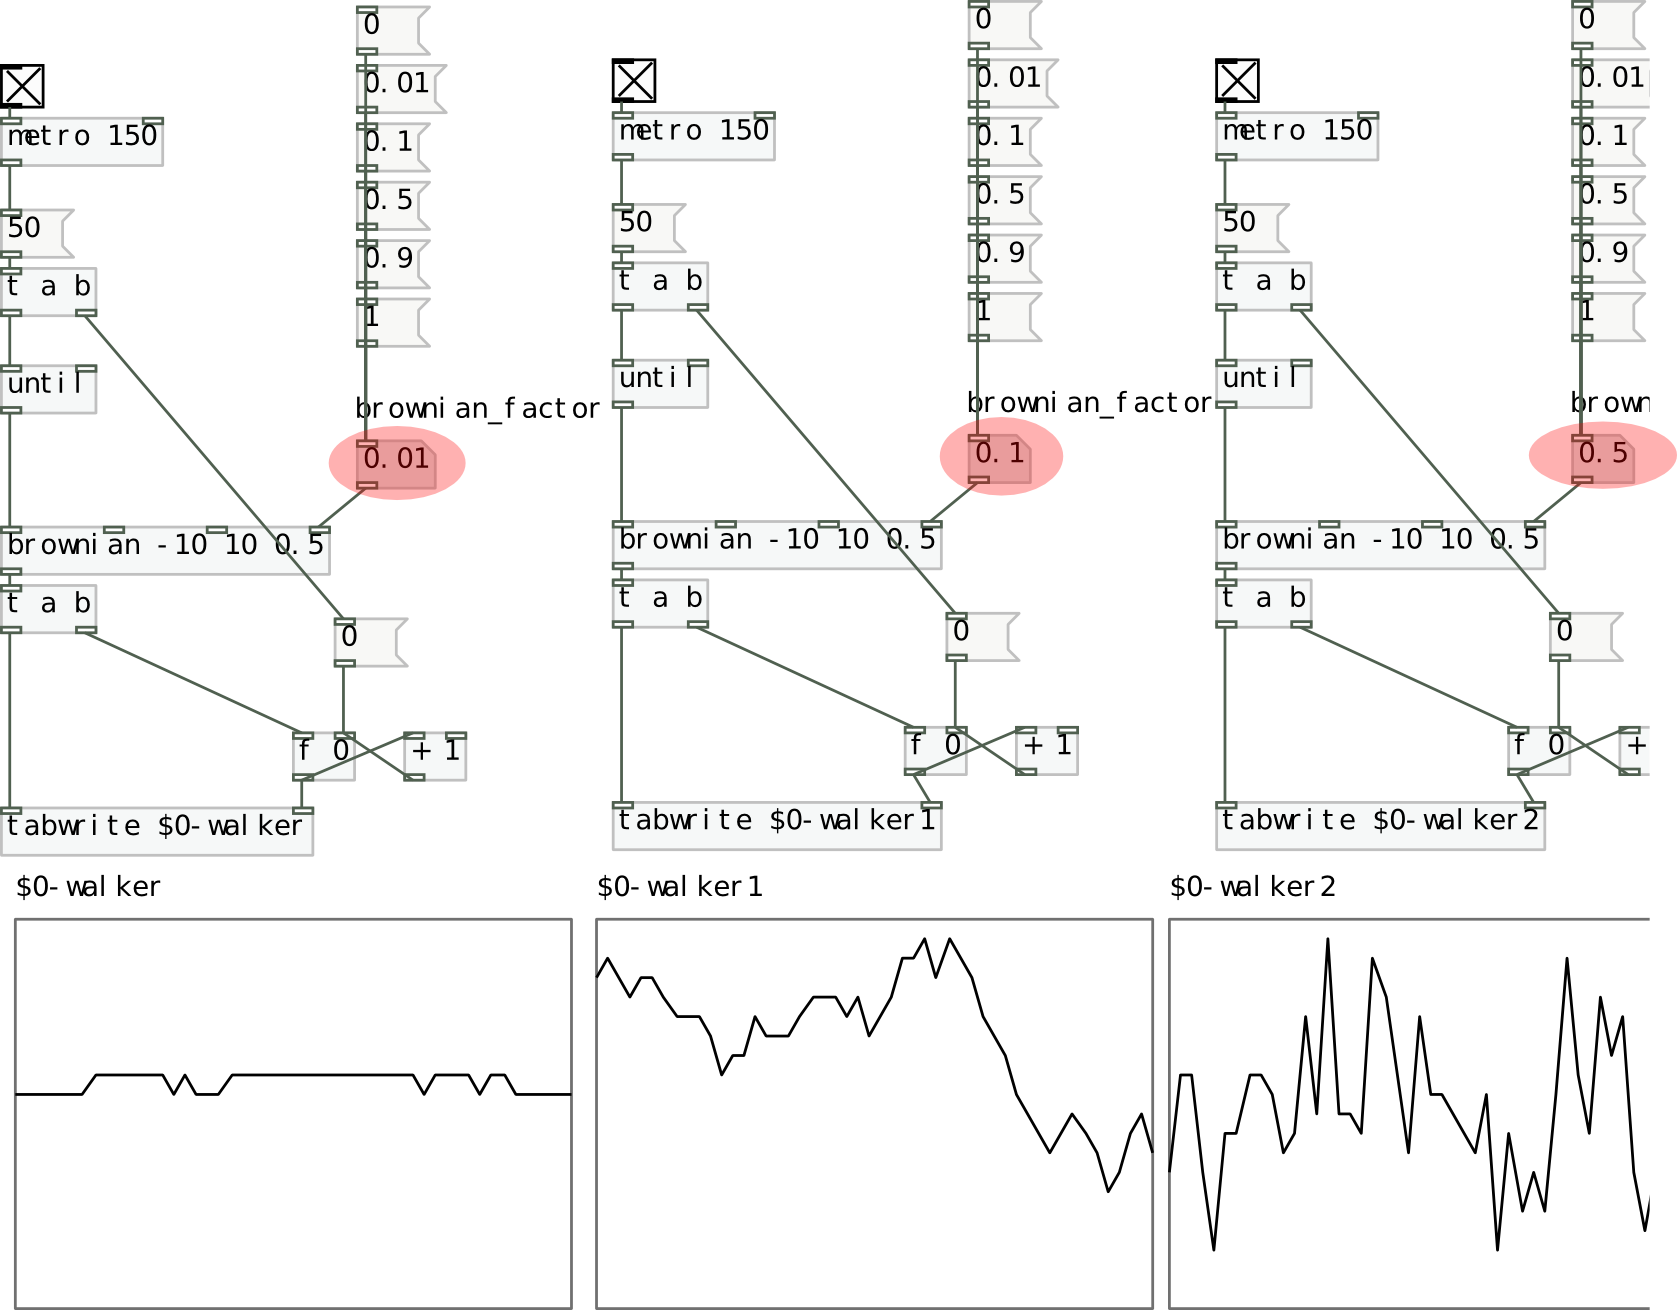
\includegraphics[scale=.6]{brownian-exemplo}
\caption{objeto [brownian] com diferentes valores de fator de brown}
\label{brownian-exemplo}
\end{figure} 

É possível comparar diferentes comportamentos de [brownian] observando
a figura \ref{brownian-exemplo}, onde vemos três objetos [brownian] com
os mesmos parâmetros de inicialização, cada um escrevendo os resultados
em diferentes arrays de 50 elementos. A única diferença entre os 3 está 
no fator de brown, assinalado em rosa (0.01 , 0.1 e 0.5 respectivamente).
Musicalmente, um baixo fator de brown aplicado a durações entre notas
possibilita a emergência de padrões rítmicos bem estabelecidos com 
pequenas variações. Quando aumentamos gradualmente o fator de brown, ouvimos
uma transição rumo a uma instabilidade rítmica e a quebra de padrões. 
O objetivo desse gerador é se aproximar da performance do músico real.
O objeto [sinc-audioanalise] analise o áudio de entrada estimando os valores de duração entre notas.
Esse valores são enviados a [sinc-calc-ritmo] que faz uma estimativa do grau
de instabilidade.
O grau de instabilidade rítmica influencia direto o comportamento do fator de brown, de acordo
com a definição do cenário de interação a que se propõe. O cenário pode definir, por exemplo, que
um ritmo estável do músico (baixa instabilidade), provoque um comportamento rítmico instável
do gerador (fator de brown alto).



 \begin{figure}
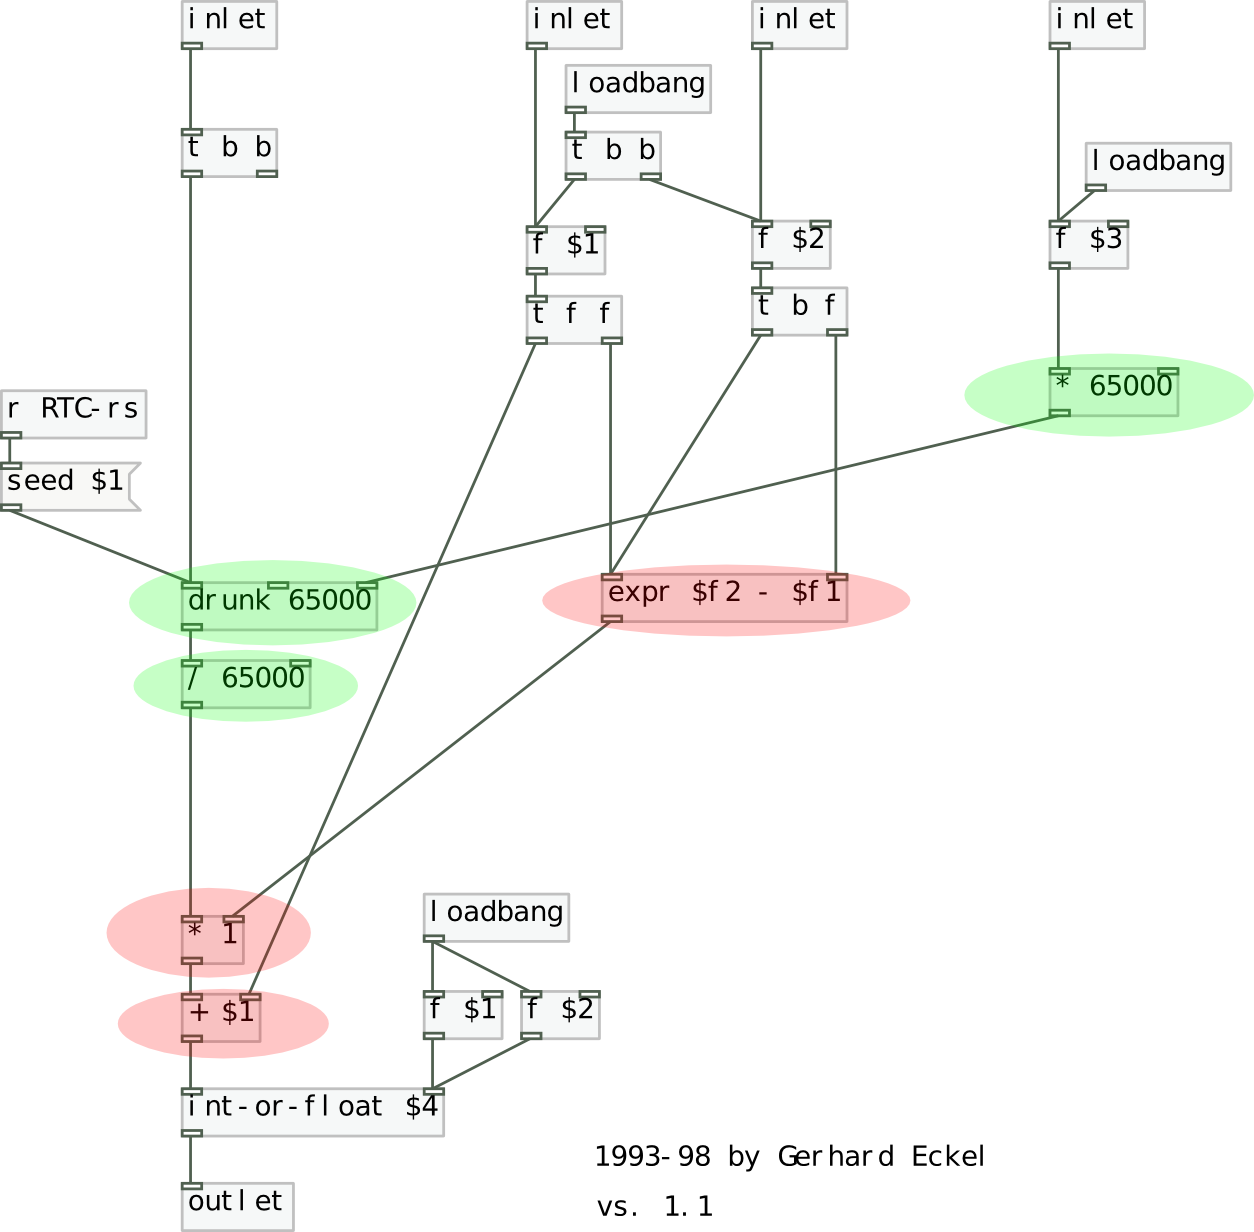
\includegraphics[scale=.6]{brownian}
\caption{[brownian]}
\label{brownian}
\end{figure} 


Na figura \ref{brownian} vemos a composição interna do objeto [brownian] onde temos elementos
grifados com a cor verde e outros com a cor rosa. Se trata de duas partes
distintas do patch, a parte com a cor verde, representa o controle dos
parâmetros do objeto [drunk] que é a implementação de um modelo de \textit{random-walk}
no Pd. A área destacada em rosa mostra uma sequência de objetos que 
escalonam o resultado dentro da amplitude de valor mínimo (\$1) e máximo (\$2).

O objeto [drunk] pertence a biblioteca Cyclone, que tem como objetivo
implementar objetos compatíveis entre Pd e MAX. O objetivo de [drunk] é
retornar números randômicos dentro de uma escala variável. A distância
entre cada número randômico é definida pelo valor da terceira entrada
de [drunk]. Essa variável define o maior número de passos possível entre 
dois resultados de [drunk]. 

Os objetos [brownian] e [drunk] são muito úteis para a composição 
interativa por permitirem a variação dos parâmetros do algoritmo
em tempo-real. Essa funcionalidade é usada em SINCOPA em outros geradores
melódicos e de dinâmica.


\subsection{Boids}

Boids é o nome de batismo de um algoritmo simples, usado na simulação de deslocamento
de grupos de animais na natureza, como cardumes de peixe e bandos de pássaros.
Esse algoritmo foi inventado pelo animador de computação gráfica Craig Reynolds.
O nome é um trocadilho referindo-se a ``birds'' pronunciado com sotaque de Nova York.
Na definição, cada boid é um indivíduo pertencente a um coletivo.

Através da observação do deslocamento de bandos de pássaros, Reynolds conseguiu
descrever alguns padrões de deslocamento espacial dos indivíduos dentro do grupo.
É um modelo baseado no conceito de que cada indivíduo em um coletivo segue simples regras
comportamentais em relação aos seus vizinhos, e que a interação dessas regras
produz a propriedade emergente de um grupo coordenado.
Brevemente, as regras internas do algoritmo são:

\begin{enumerate}
 \item Os boids tentam voar em direção ao centro de massa dos outros boids vizinhos;
 \item Boids tentam manter uma pequena distância dos outros objetos (incluindo outros boids);
 \item Cada boid tenta sincronizar sua velocidade com boids vizinhos; 
\end{enumerate}

Basicamente, a cada instância temporal, os parâmetros espaciais de cada boid são re-calculados
levando em conta um centro de atração e os comportamentos dos vizinhos.
Esse algoritmo tem potencial enquanto gerador de material musical numa perspectiva de interação.

\begin{figure}
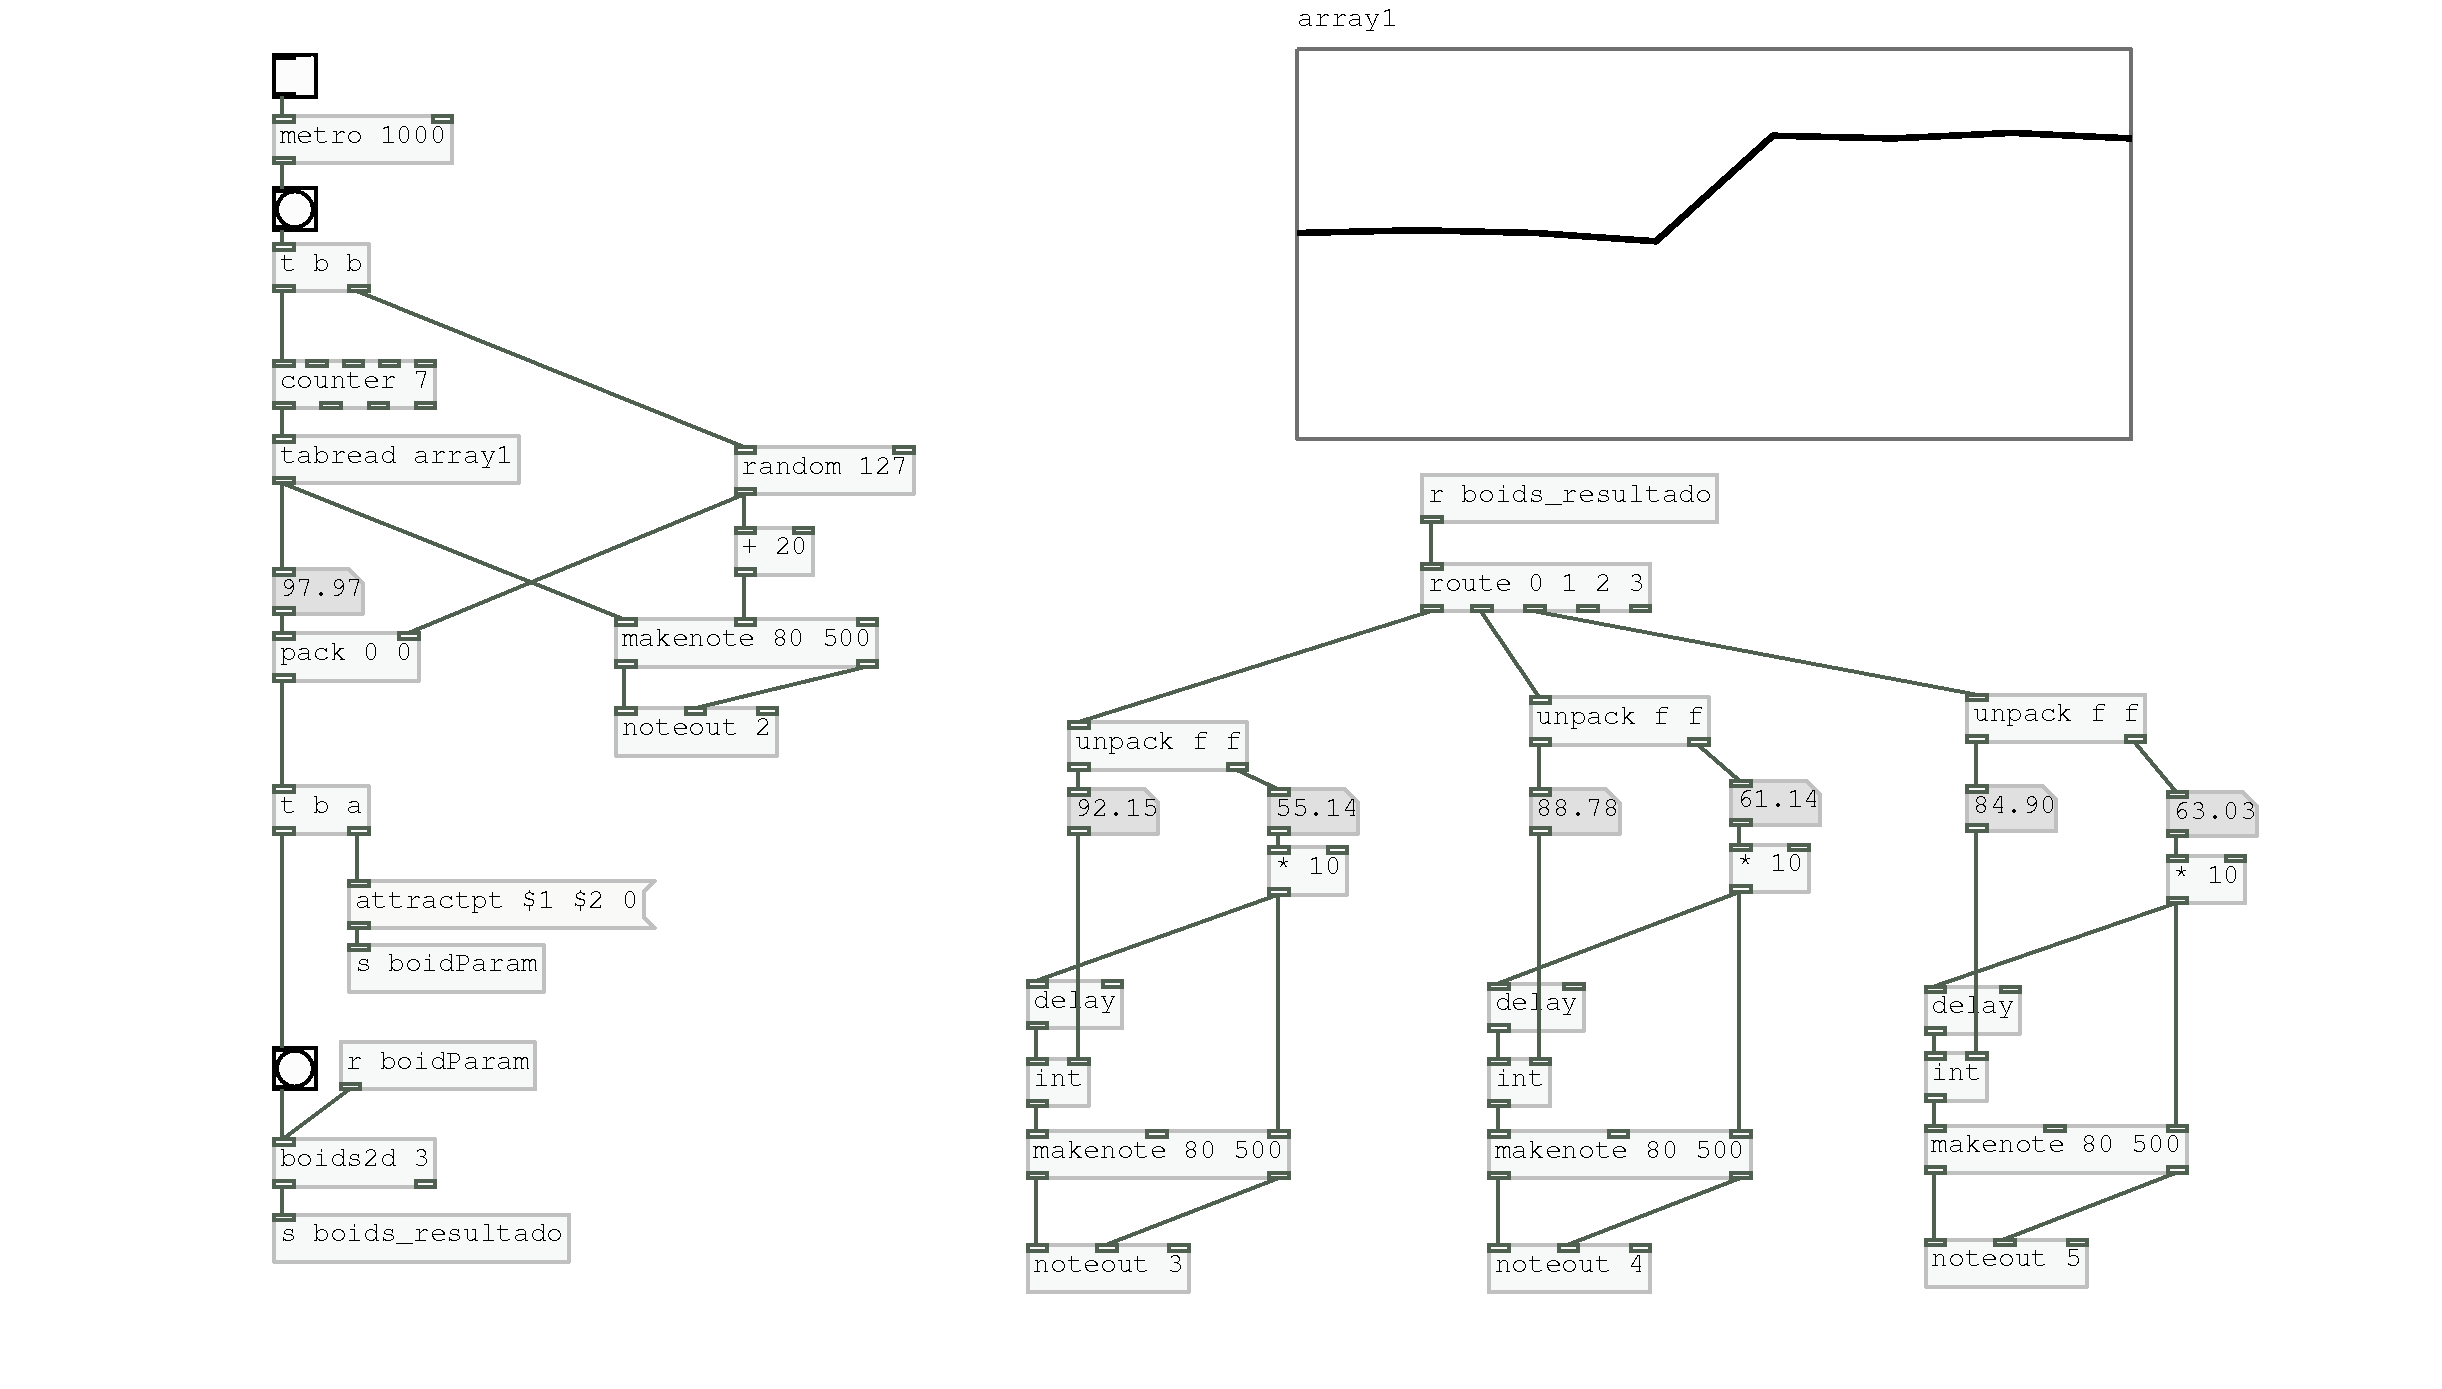
\includegraphics[scale=.6]{midi-boid}
\caption{Objeto [boids2d] controlando 3 boids geradores de notas MIDI}
\label{midi-boid}
\end{figure}  


O Pd-extended traz uma implementação de boids na forma do objeto [boids2d] que recebe mensagens de parâmetros
de comportamento global, parâmetros do centro de atração e calcula as novas posições XYZ de cada
boid. No caso de uma aplicação musical desse algoritmo foi pensado num primeiro momento que as frequências
podem representar o eixo X e o tempo de execução o eixo Y. 
Na figura \ref{midi-boid} vemos um array que representa a entrada de alturas do músico. Esse array atua como
o ``líder'' que é seguido por outros três boids. A altura e a velocity são enviadas para o objeto [boids2d],
que retorna o valor de altura e intensidade dos três boids que representam três vozes. Cada voz é escrita
em um canal MIDI.


Os parâmetros de controle de comportamento do algoritmo interno em [boids2d] são controlados através de mensagens
com símbolos e valores.
Cada parâmetro tem uma frase que explica a influência no comportamento global. Nesse experimento,
apenas o parâmetro \textit{attractpt} é atualizado em tempo-real, enquanto todos os outros são
fixos.

\begin{figure}
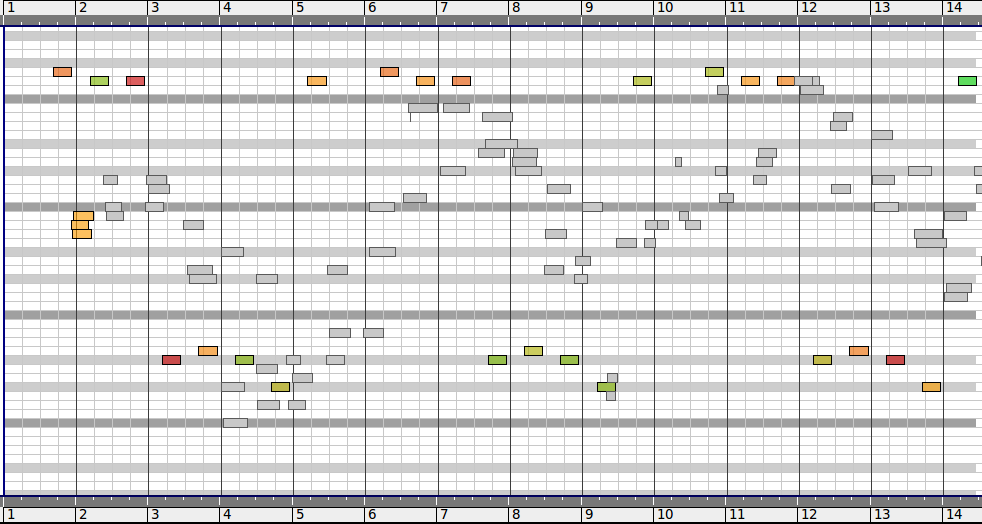
\includegraphics[scale=.4]{boids-pianoroll}
\caption{Visão de resultado de 3 boids seguindo perfil melódico no piano-roll}
\label{boids-pianoroll}
\end{figure} 

O resultado do patch visto na figura \ref{midi-boid} pode ser visto
na figura \ref{boids-pianoroll}. Onde vemos que as notas executadas pelo array estão destacadas
em cores, enquanto que as notas geradas pelos boids estão em cinza. Podemos notar um certo ``atraso''
 na ação de seguir o ``líder''. Esse atraso pode ser alterado através dos parâmetros, por exemplo
o parâmetro \textit{inertia} que controla essa ``disposição'' para mudar de velocidade e de direção
está muito baixo, a medida que aumentamos esse valor iremos notar
os boids seguindo com mais rapidez o ``líder''.
O efeito musical é uma textura que varia de uma polifonia densa e aparentemente disconexa até uma 
heterofonia radical, a depender dos parâmetros de comportamento.

\section{Discussão}

O recorte da pesquisa foi o desenvolvimento de ferramentas para composição
interativa entre instrumentos tradicionais e computadores. 
Nesse sentido apresentamos algumas soluções para geração de material musical sob
o paradigma da interação com um músico humano. O foco do objeto
de pesquisa na composição interativa proporcionou que o resultado técnico
fossem ferramentas genéricas, modulares e re-utiliźaveis. 
O código em desenvolvimento de SInCoPA\footnote{Disponível em: www.github.com/cristianofigo/sinc\_abs} 
é licenciado e distribuído sob a licença GNU/GPL\footnote{
Disponível em: http://www.gnu.org/licenses/gpl.html} e vem sendo utilizado em instalações audiovisuais e
performances de música eletroacústica interativa no grupo de pesquisa Poéticas tecnológicas da UFBA. 


\section{References}



\bibliographystyle{sbc-template}
\bibliography{biblio}

\end{document}
